\chapter{Immersive Projection Technology: from Stereoscopy to Multi-stereoscopic}
\label{chapter:multistereo}
\minitoc

\section{Introduction}
In this study we experimentally created special interaction situations to examine the perceptual conflicts generated by the dual-presence of the real and virtual visual and audio stimuli. In a two-user scenario, participants performed an object-picking task according to three types of instructions (verbal, gestural or multimodal instructions) given by an experimenter. This co-located experimenter was also virtually present by an avatar in the virtual world to enable face-to-face interactions with the participants. Our goal was to observe to what extent the perceptual conflicts induced by the dual-presence of the experimenter can be integrated without significantly altering the performance of the participants. For that we studied the influence of such perceptual conflicts on participants' choice of collaborator (whether they interacted with the avatar or the real experimenter) and on their task efficiency.

We carried out an experiment to examine users' reaction to the dual-presence caused by the simultaneous virtual and real stimuli, and to analyze whether the perceptual conflicts mentioned above would make it difficult to have a face-to-face interaction via an avatar with a multi-user projection-based immersive display.

In a two-user scenario, we asked the participants to complete an object-picking task under the instructions given by an experimenter who was co-located in the same immersive device. In the virtual world, the experimenter was present via an avatar in a room with some floating targets. Participants should choose between the two forms of collaborator in order to know which target to pick. We intentionally created situations in which these two forms of collaborator were always comparable for the participants by assuring there was also a virtual object in the pointing direction of the real experimenter (see Figure~\ref{fig:2_demo}). By recording the target ID chosen by the participants, we could extract their choice of collaborator. In the meanwhile, different types of instructions (deictic gestures and/or verbal commands) were given to observe the influence of perceptual conflicts on different sensory channels (visual and auditory).

\begin{figure}[ht]
  \centering
  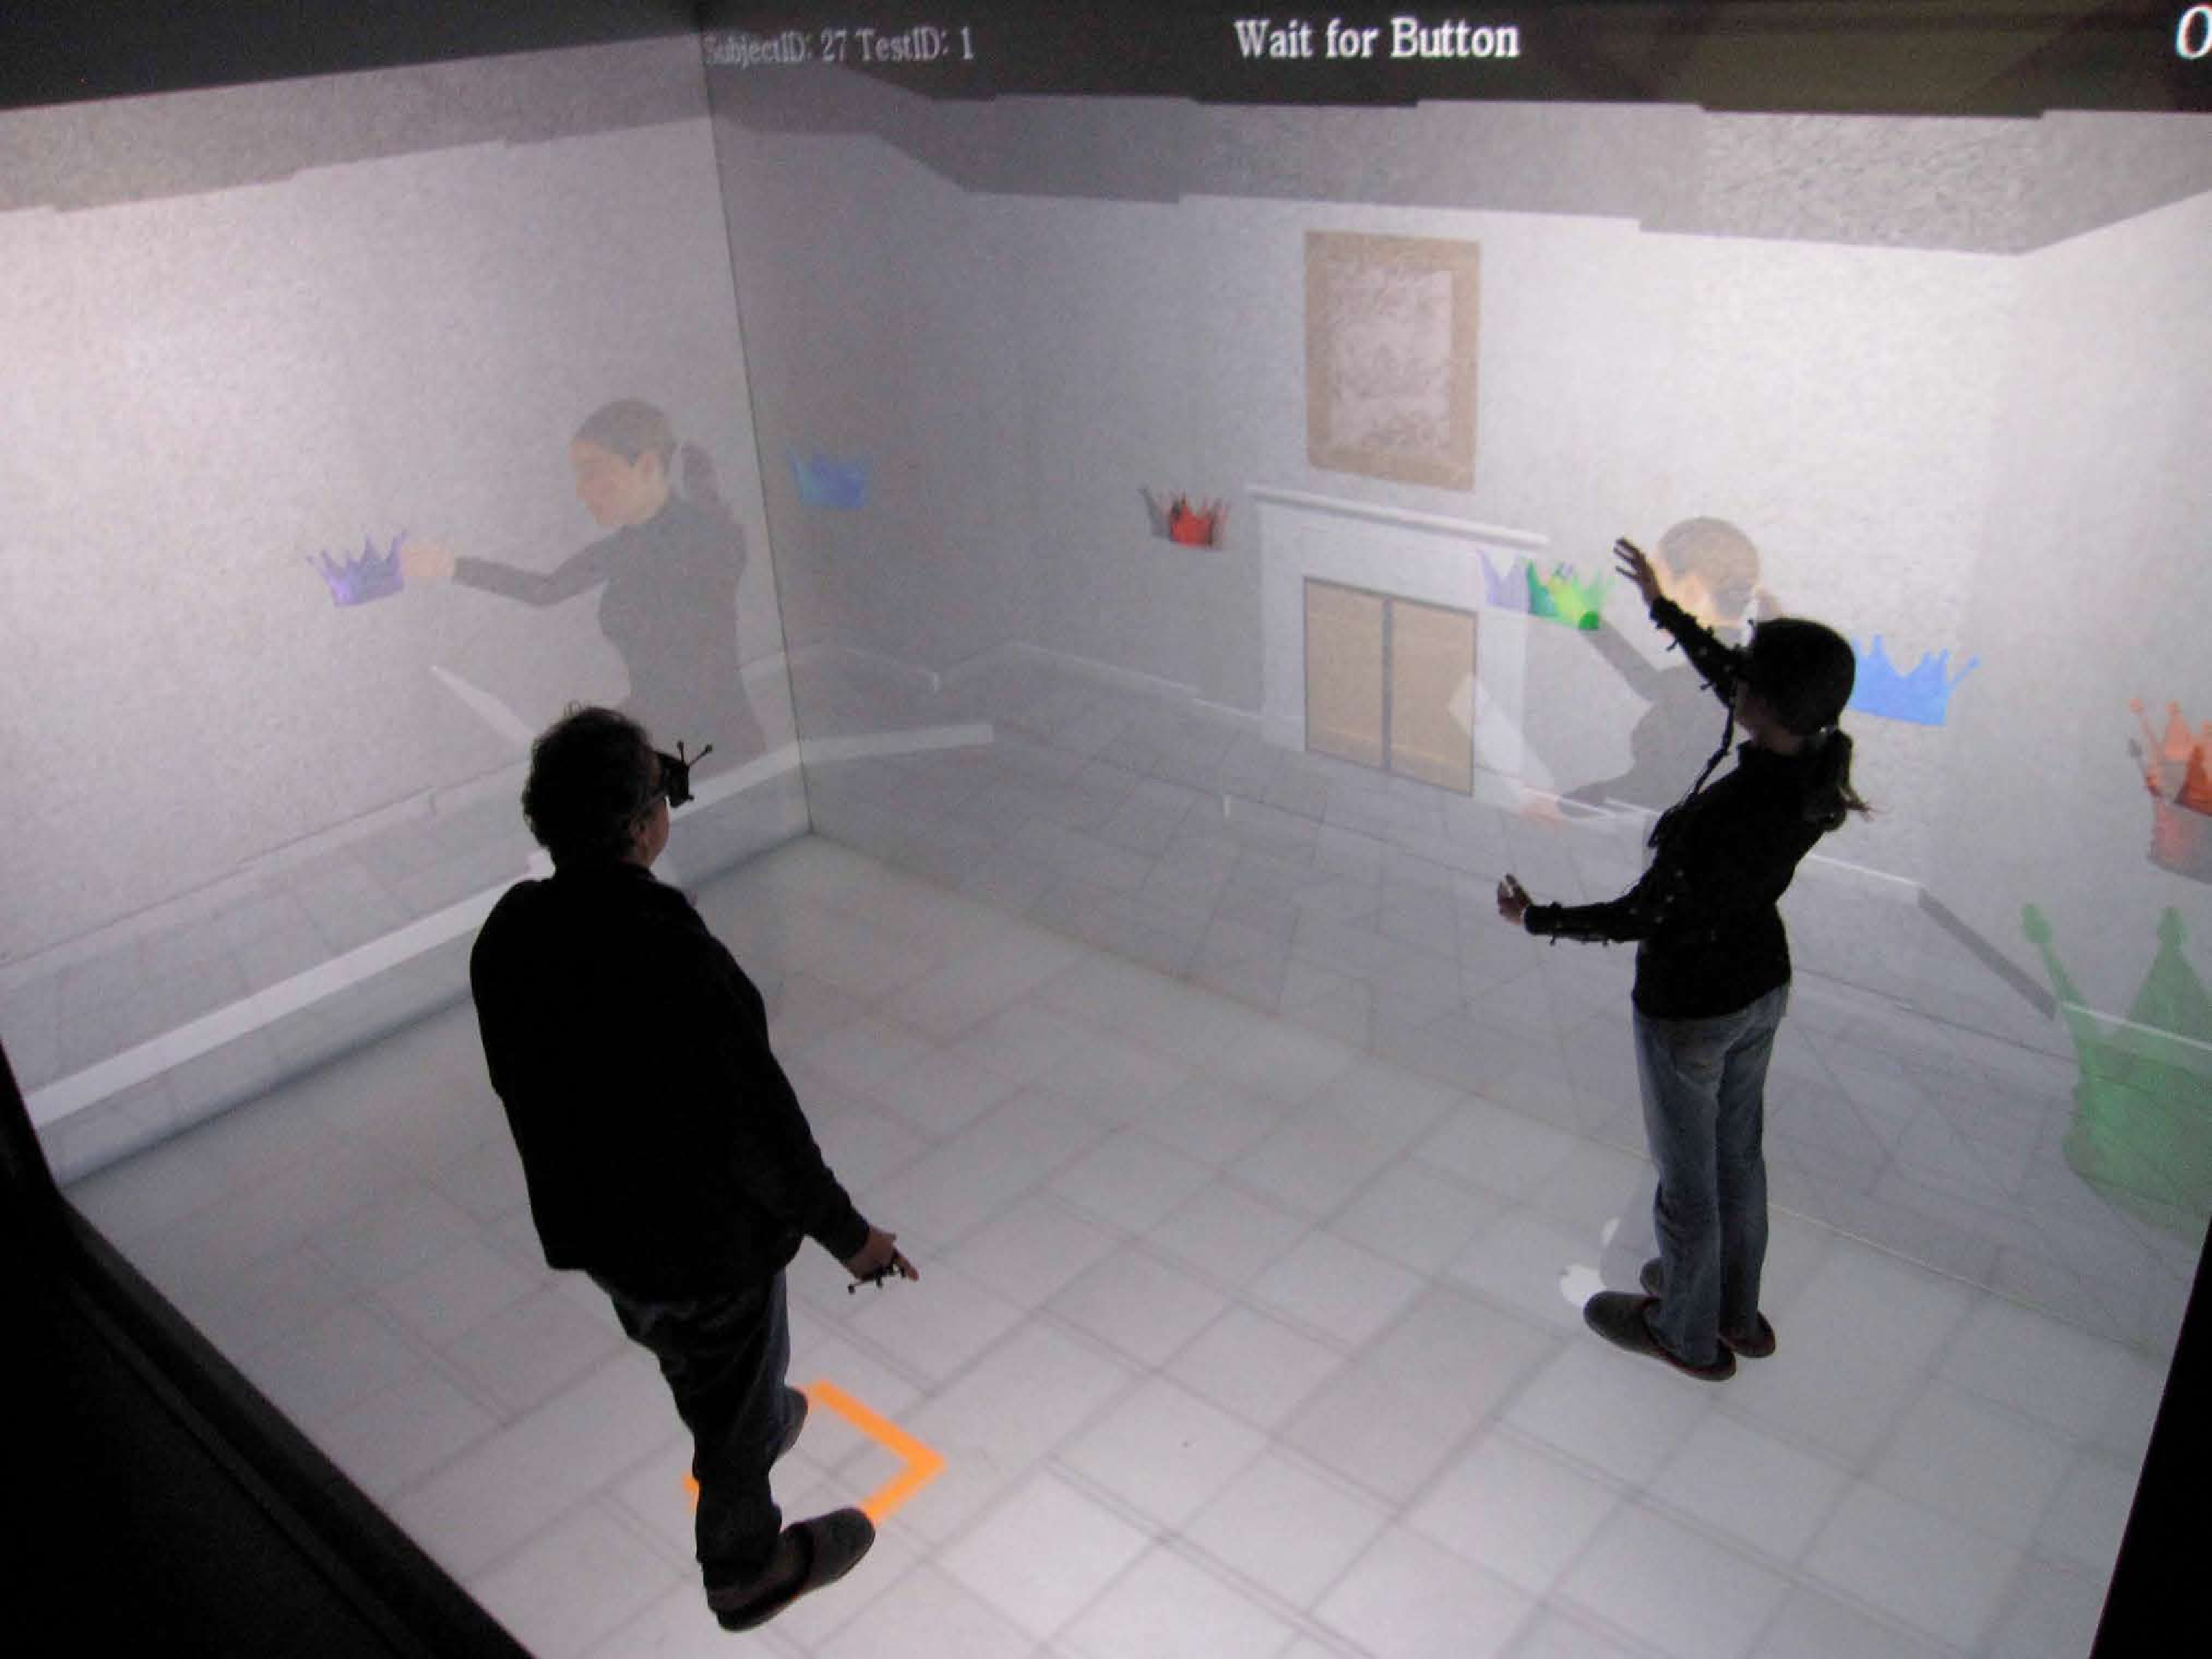
\includegraphics[width=0.9\textwidth]{figures/2_demo}
  \caption{\label{fig:2_demo}The 3D view of the participant and that of the experimenter were superimposed on the multi-stereoscopic display. The participant faced the dual-presence of the experimenter and her avatar, while from the experimenter's viewpoint, the avatar was co-localized with her physical body.}
\end{figure}

Two independent variables were chosen: the angular distance between the real experimenter and the avatar, and the type of instruction (verbal-only, gesture-only or multimodal) given by the experimenter. We believed that these variables may interfere with user's collaborator choice and task performance. For example, the proximity of the real experimenter and the avatar may increase the level of visual conflicts and users may be more disturbed by gestural instructions than verbal ones.


\section{Stereoscopy, Human's Visual System}


\section{Multi-stereoscopy}
Most projection-based displays can only support one fully tracked active user, other co-located users can only share the same point of view with distorted images and participate passively in the collaborative task \citep{Bayon2006Multiple}. This visual distortion impedes users' collaborative spatial judgments by impacting the perception of depth and direction in the virtual world \citep{Pollock2012Right}. To avoid visual distortion, different approaches have been explored to provide individual stereoscopic views for multiple co-located users with projection-based display. For example, Simon proposed a multi-viewpoint images technique \citep{Simon2007MVI} which projects different images from multiple viewpoints corresponding to the viewing positions of multiple users, and combines them to a single image on the screen. Users can only get a correct stereoscopic view from predefined position without head tracking, so with static images the interactions that they can have are limited. Other display solutions can also provide individual stereoscopic views like the volumetric display \citep{Grossman2008Volum} and holographic display \citep{Lucente1997Holo}. However, these techniques can only be applied to non-immersive context with limited workspace.

\subsection{Image Seperation Technique}
In order to have relatively large separate adaptive stereoscopic images for multiple users, time-multiplexing techniques become a working solution. Efforts have been made since 1997, for example, \citet{Agrawala1997TRW} designed a prototype of a responsive workbench to provide two tracked users with independent stereoscopic views without distortion. Later on, \citet{Kunz2002TSC} used a pair of shuttered LCD projectors to generate an active stereo display and then \citet{Frohlich2005MultiViewer} extended this shuttered display to support two to four users with better performance in terms of perceived flicker, brightness of each view and crosstalk. This technique makes it possible for a single screen to support more than one stereoscopic view. Images for different users are separated by active shutter glasses while the separation of the images for the left and right eye is ensured by passive polarized filters. In 2011, \citet{Kulik2011CSS} even developed a projection-based stereoscopic display for six users by using six customized DLP projectors. With each user having an independent stereoscopic view combined with real-time head tracking, more complex collaboration scenarios can be implemented for a group of co-located users.

Besides the development of display technology, various interaction techniques have also been proposed to make co-located collaboration in multi-user projection-based systems easier and more efficient, such as the bent pick ray \citep{Riege2006Bent} and the see-through techniques \citep{Argelaguet2010STT}. However, these interaction techniques focus solely on situations where users are side-by-side. Direct face-to-face collaboration in projection-based display system is supposed to be impossible \citep{Salzmann2009CIC}. Therefore here we tried to study the possibility of having co-located face-to-face collaboration by investigating users' reaction to the perceptual conflicts raised with the dual-presence of the avatar and the real person.

\subsection{Application for Collaborative Work}
Large projection-based displays can be an effective solution to support co-located collaboration in immersive CVEs. Especially, with the multi-stereoscopic projection-based setup as used by \citet{Salzmann2009VRPointing}, multiple users can collaborate side-by-side and interact with a virtual object in front of them with individual stereoscopic views of the virtual scene. However, as indicated by \citet{Salzmann2009CIC}, certain tasks that require face-to-face interaction between users cannot be applied directly within projection-based displays due to occlusions if an object is located in the middle of the users. In this case, if we want to benefit from the advantages of co-located collaboration in projection-based multi-stereoscopic systems for face-to-face tasks as in the side-by-side situations, we should prevent the users from working directly with each other.

Thus a possible solution is to introduce an avatar animated by real-time body motion capture for each user, and let each user work with the other users' avatars instead of the real person. In this case users' spatial relationship (relative position and orientation) in the virtual world is no longer constrained by the one in the physical workspace, they can be facing each other in the virtual world while physically side-by-side. This avatar-based approach enables complicated tasks that require both face-to-face and side-by-side interactions in projection-based multi-user system. For example, a car assembly task may contain two phases: during the first phase, users are on the same side of the model. They discuss and work together to repair a specific part of the car. Then in the second phase, they need to be at opposite sides of the car, and consequently have different viewpoints in the virtual world. Within this scenario one user can guide the other to properly fix a seat within the car cockpit. So with our avatar-based approach, they can switch between different spatial configurations without interrupting the ongoing task by using virtual navigation techniques.

However, with the solution proposed above, sometimes users may still enter each other's field of view when they work with the avatars. What is more, during a collaborative task, the communications between collaborators are usually conducted in a multimodal way \citep{Paggio2005Multimodal, Ennis2010Seeing} including verbal and non-verbal modalities \citep{Bailenson2002Gaze, Dodds2011Talk}, especially deictic gestures to refer to objects or places. So during a two-user co-located collaboration scenario, with the dual-presence of virtual and real information, users having multimodal interactions may encounter different perceptual conflicts both in the visual and audio modalities. For example (see Figure~\ref{fig:2_inconsistency}(a)), if user B points to an object for user A (from user B's viewpoint, he/she is pointing at a cube), user A may be confused by seeing both user B and his/her avatar doing the pointing gesture, and it may be problematic when there is another virtual object in the pointing direction of user B. Furthermore, normally the verbal communication between co-located users is conveyed by direct conversation without using headphones. As shown in Figure~\ref{fig:2_inconsistency}(b), user A is interacting with user B's avatar, but the vocal information comes from the real user B in a different direction. This kind of visual-audio inconsistency \citep{Di2009Recalibration, Spence2013Just} may be disturbing for users to concentrate on their collaboration.

\begin{figure}[ht]
  \centering
  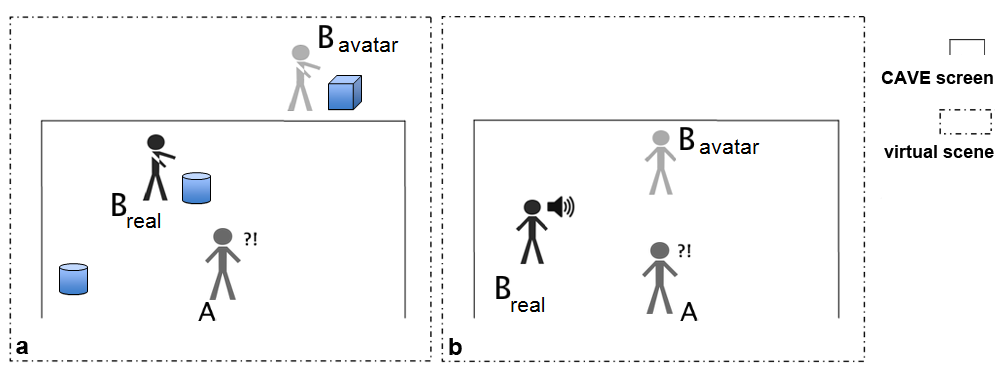
\includegraphics[width=\textwidth]{figures/2_inconsistency}
  \caption{\label{fig:2_inconsistency}Illustration of perceptual conflicts with a two-user scenario; user A interacts with avatar of user B: (a) Visual conflict occurs when user A simultaneously perceives the real user B and B's avatar pointing to different virtual objects. (b) Visual-audio conflict occurs when user B and the avatar are not at the same position.}
\end{figure}


\subsection{Dual Presence}
With multi-stereoscopy technology, novel projection-based immersive systems now can support multiple users by providing each one with an independent stereoscopic view of the virtual scene. When users work face-to-face, they may have an incorrect view if objects are located between them. In this case, avatars can be introduced to enable face-to-face interaction in the virtual world whereas they are side-by-side in the real device. As a consequence, such multi-user systems provide the users with a new kind of perceptual immersion and related cognitive experiences, because users must handle both information from the real world (i.e., other users' bodies) and those from the virtual scene (i.e., other users' avatars) at the same time.

Avatars have been used as media for multi-user communication in both remote and co-located use of immersive CVE, but the dual-presence of users and their avatars in the same immersive device for face-to-face interaction has not yet been addressed. We do not intend to create such dual-presence to test user's preference between real person and the avatar, but to observe users' reaction to different perceptual conflicts and to study if our avatar-based approach is sufficient to support face-to-face co-located collaboration in a multi-stereoscopic immersive display system.

Besides the development of display technology, various interaction techniques have also been proposed to make co-located collaboration in multi-user projection-based systems easier and more efficient, such as the bent pick ray \citep{Riege2006Bent} and the see-through techniques \citep{Argelaguet2010STT}. However, these interaction techniques focus solely on situations where users are side-by-side. Direct face-to-face collaboration in projection-based display system is supposed to be impossible \citep{Salzmann2009CIC}. Therefore here we tried to study the possibility of having co-located face-to-face collaboration by investigating users' reaction to the perceptual conflicts raised with the dual-presence of the avatar and the real person.


\section{User Study}
We conducted an experiment to study users' behavior for the co-located use of multi-stereoscopic display system. We want to see which reference frame (real vs. virtual) the participants choose and their task performance according to different experimental conditions.

During a two-user scenario of a collaborative task, the participant and an experimenter (i.e., one of the authors) were situated in the same immersive environment (a double-stereoscopy CAVE-like system). In the virtual scene, they were co-localized in a room about the size of the real set-up with some floating crowns (see Figure~\ref{fig:2_virtual_room}). The task for the participant was to reach one of the crowns according to the instruction given by the experimenter during each trial.

\begin{figure}[ht]
  \centering
  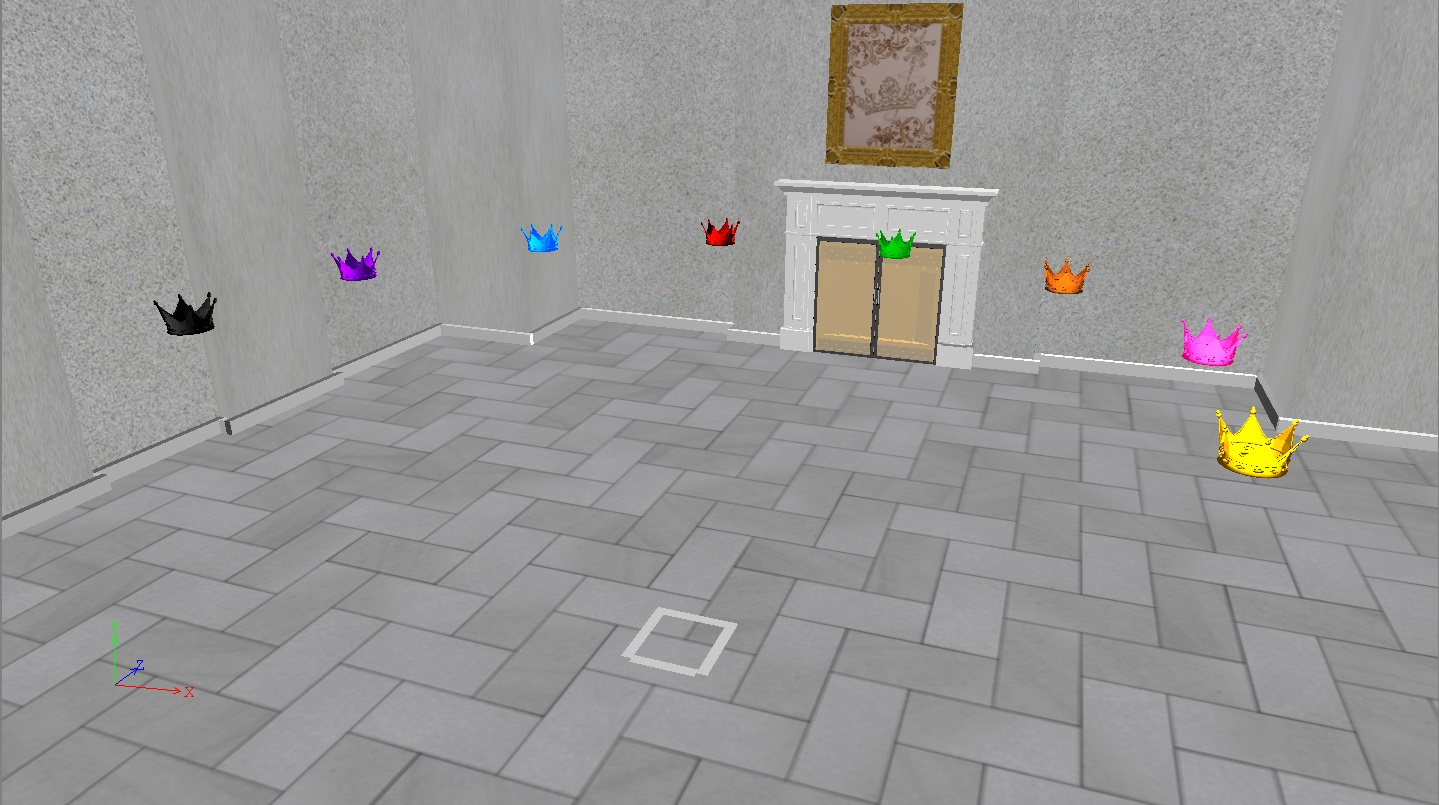
\includegraphics[width=0.8\textwidth]{figures/2_virtual_room}
  \caption{\label{fig:2_virtual_room}Front view of the virtual scene used for the experiment.}
\end{figure}

\subsection{Participants}
27 participants (23 men and 4 women) passed our experiment. The average age is 26 years (standard deviation 4.8 years).
A large number (23) of the participants were people with a computer science background. All participants filled out a background questionnaire, which was used to gather demographic information such as their level of computer skills, experience with video games and with virtual reality devices, and some other personal statistics (e.g., age, dominant hand, etc). Among these participants, 26 were right-handed and one person was left-handed. All participants used their dominant hand to perform the designation task and were naive with respect to the experimental setup and purpose of the experiment.

A specific avatar was designed to match the experimenter's profile like the height, the clothes and the face (without facial expression) so that the real and virtual visual stimuli were comparable (see Figure~\ref{fig:2_avatar}(a)). In order to make the avatar follow user's physical body movements, we used a full-body motion capture system to map the experimenter's upper body motions to her avatar. A flystick was also provided for the experimenter to trigger the timer for task performance measurements (see Figure~\ref{fig:2_avatar}(b)).

\begin{figure}[ht]
  \centering
  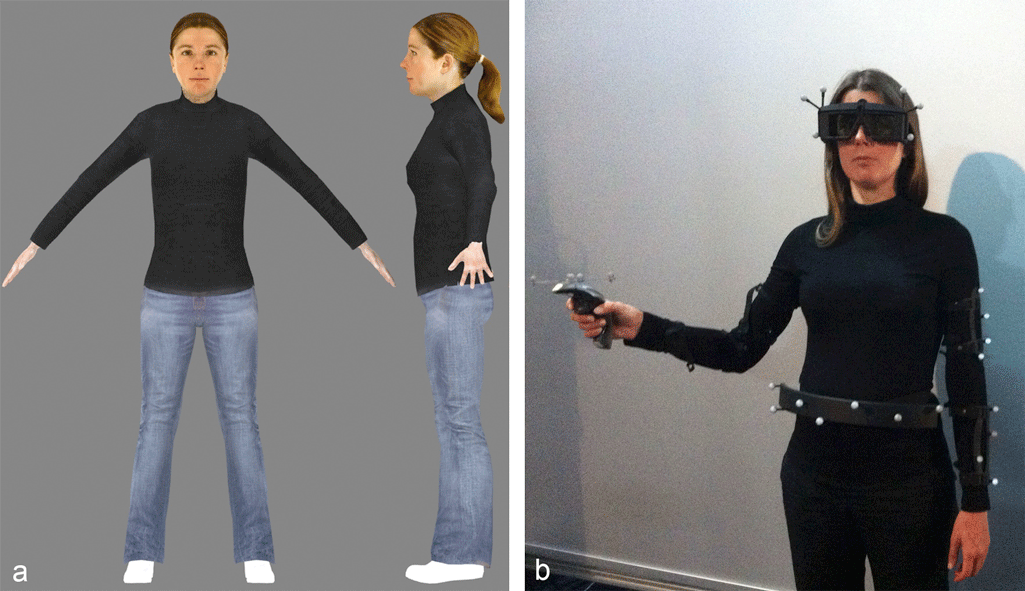
\includegraphics[width=\textwidth]{figures/2_avatar_photo}
  \caption{\label{fig:2_avatar}(a) The avatar of the experimenter used in the experiment. (b) The experimenter wore a motion-tracking suit to map upper body movements to the avatar.}
\end{figure}

No avatar was provided for the participants since we did not study the visual perception of the experimenter. The participants wore a pair of tracked shutter glasses to see stereoscopic images and a tracker on one hand to enable direct interaction with virtual targets by hand movements.

\subsection{Experimental Condition}
In this experiment, we manipulated two independent variables to study their impact on participants' choice of collaborator and task performance. Here is a detailed description of these independent variables:

Delocalization angle: As shown in Figure~\ref{fig:2_floor}(a), at the beginning of each trial, the participant should stand at a given point (the white square at the center of the circle) to wait for the experimenter's instruction. Around this starting point, seven predefined positions were distributed on a half circle with a radius of two meters symmetrically from the left to the right of the CAVE workspace (smaller white squares). For each trial, the experimenter and her avatar were located on one of these seven positions which were equidistant to participant's standing point, so the delocalization level between the real collaborator and her avatar can be measured by the angle between two segments started from the center of the circle (where the participant stood) and ended respectively at the positions of the experimenter and her avatar (see Figure~\ref{fig:2_floor}(b)). This delocalization angle has seven different values from 0$^\circ$ to 180$^\circ$ with an interval of 30$^\circ$ given the configuration of the chosen seven locations.

Instruction type: Interaction between users usually involves verbal and gestural modalities. In order to inspect their impact on co-located collaboration with dual-presence, we defined three deictic instruction groups: verbal-only instruction, gesture-only instruction, and multimodal (gesture and verbal) instruction. Each instruction group was then divided into two sub-groups to take into consideration the possible left-right effect. Finally we got 6 different instruction groups as indicated in Table~\ref{tab:instruction_type}. To be more precise, the target object (the crown) indicated by the experimenter was the nearest one (e.g., ``Go to the crown on my left" indicated the closest crown on the left side of the experimenter when there were more than one presented target). To make sure that ambiguities were present no matter the actual spatial configuration, there was always one crown on the left-hand side and one on the right for each of the seven predefined positions of the experimenter.

\begin{figure}[ht]
  \centering
  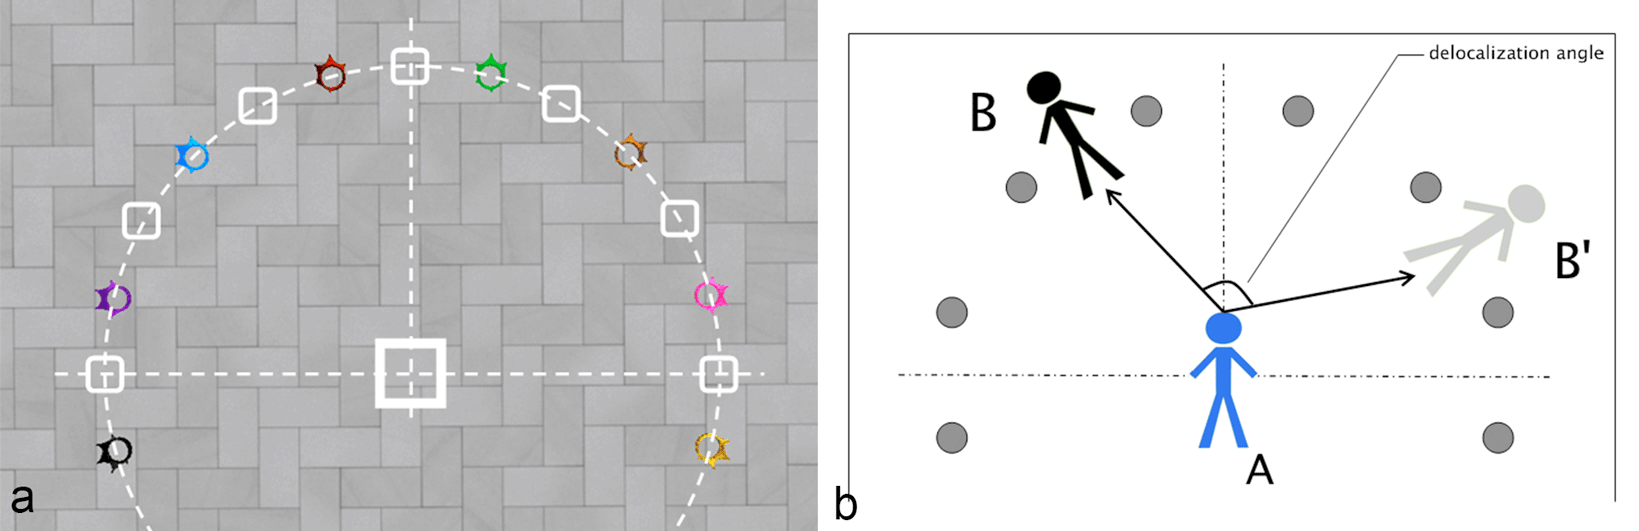
\includegraphics[width=\textwidth]{figures/2_floor}
  \caption{\label{fig:2_floor}(a) The top view of the virtual scene indicates the configuration of the virtual room and predefined positions for participants and their collaborator. (b) An example of the delocalization angle due to the separation of the real experimenter and the associated avatar.}
\end{figure}

\begin{table*}[!t]
\renewcommand{\arraystretch}{1.3}
\caption{All six types of deictic instructions given by the experimenter for the object-picking task.}
\label{tab:instruction_type}
\centering
\begin{tabular}{l l l}
	\hline
	No. & Type & Example \\
	\hline
    1 & Gesture-only & Point to the crown on the left. \\
    2 & Gesture-only & Point to the crown on the right. \\
    3 & Verbal-only & ``Go to the crown on my left." \\
    4 & Verbal-only & ``Go to the crown on my right." \\
    5 & Multimodal & ``Go to the crown on my left" (point to the left). \\
    6 & Multimodal & ``Go to the crown on my left" (point to the left). \\ \hline
\end{tabular}
\end{table*}

We defined the combination of the experimenter's position and her avatar's position as the spatial configuration of the trial. Since there were seven possibilities for both positions (Figure~\ref{fig:2_floor}(a)), this resulted in 49 different spatial configurations in total. Due to time limitation, there were too many spatial configurations for each participant to test all of them, so we distributed these configurations among all the participants with each person testing a subset and covered all the conditions at a global level. We grouped the spatial configurations by the delocalization angle that they formed, and each participant passed one configuration for each delocalization angle with all six types of instructions. In order to offset the interaction affect between the delocalization level and the instruction type, all the trials for each participant were presented in a randomized order.

Finally, in this experiment, participants moved directly in the virtual scene through natural walking with a scale of one to reach the target object. This choice was taken in order to make the evaluation independent with any navigation paradigm to avoid warping the results because some participants may be more familiar than others with virtual interactive navigation techniques.


\subsection{Protocol}
First, each participant was invited to sign an informed consent and then an overview of the experiment was provided. This experiment was conducted in three main phases for each participant:

\begin{itemize}
\item Presentation stage: We introduced the main procedure of the experiment, the nature of instructions and the duration of each step to the participant. A pre-questionnaire about cybersickness was filled out.
\item Learning stage: Six randomized trials were given for the participants to get familiar with the experimental setup.
\item Experimental stage: The participant accomplished collaborative tasks under the instructions of the experimenter. The experimental stage for each participant was the same except each one of them tested a subset of all the spatial configurations. Each participant tested seven spatial configurations with all six types of instructions, so in total 42 trials. The working scenario was the following:

At the beginning of trial, the virtual scene was covered by a blue curtain (virtual one). We set up the curtain and asked the participant to lower the head in order to avoid the participant from seeing the experimenter and her avatar before the trial began. The participant should stay at his/her departure position and look at his/her feet until the curtain disappeared. Once the experimenter reached the required position indicated by the square on the floor (Figure~\ref{fig:floor}(a)), the system then put the experimenter's avatar at another required position to form a delocalization angle (from 0$^\circ$ to 180$^\circ$) and hid the curtain.

The experimenter read the instruction showed on a piece of virtual paper in her left hand and then indicated the target (one of the crowns) the participant should travel to by giving verbal and/or gestural instruction, and then started the timer by pushing a button on the flystick. Then a beep was delivered by a loudspeaker to inform the participant to respond. Participants were not supposed to start before the beep, otherwise the trial was not counted.

The system recorded the time when the participant left the initial position as reaction time (A participant had the right to give up and pass to the next trial before he/she reached a certain target). The system also stored the time from the moment the participant left the initial position until he/she reached a target (correct or not) as execution time.

The selected crown ID (from 1 to 8) was recorded in order to know the participant's choice of reference frame. When the experimenter and the avatar were not superimposed, they would lead the participant to different targets depending on their actual positions and the given instruction. So we recorded the selected crown ID to see which target was chosen by the participant, and then we could determine whether the participant followed the real experimenter, or her avatar, or neither of them (considered as a failure). If the participant chose to give up, the trial was also considered as a failure of the task. When the task was finished, the participant came back to the initial position and waited for the next trial.

\item Questionnaire stage: First, a post-questionnaire to evaluate the level of cybersickness was conducted. Then we tested the participants with a detailed subjective questionnaire for the collaborative task (see Appendix) and finally another questionnaire to get participants' personal information.
\end{itemize}


\subsection{Measures}
\subsubsection{Performance measures}
For each trial, we recorded reaction time (noted as RT), execution time (ET) and the total time (TT, sum of the reaction and execution time) to finish the task. Moreover, we recorded participant's choice of reference frame for each trial using the crown ID.

\subsubsection{SSQ Pre-assessment and Post-assessment}
The questionnaire used for cybersickness evaluation is Simulator Sickness Questionnaire (SSQ) (Kennedy, et al., 1993). The SSQ was administered before and after exposure to the virtual environment. The SSQ is a 16-item measure in which participants report symptoms on a scale of 0 to 3 (0 = None, 3 = Severe). Three types of symptoms are assessed: oculomotor dysfunctions (O) (eyestrain, blurred vision, difficulty in focusing), mental disorientation (D) (difficulty in concentrating, confusion, apathy), and nausea (N) (including vomiting). Unit scores (O, D, N) are weighted scores. The SSQ is a widely used measure of simulator sickness that has been shown to be a valid measure of this construct in VR research (Cobb, et al., 1999).

\subsubsection{Subjective measures}
Data were collected using a subjective evaluation questionnaire with a 4-point rating scale, ranging from 0 (do not agree at all), 1 (do not agree), 2 (neutral), 3 (agree), to 4 (fully agree). We regrouped the items into three categories according to three measured dimensions. Nine items measured the participant's confidence on the success of the task, 11 items estimated the participant's understanding of instructions, and 15 items measured participant's reaction to the dual-presence of the experimenter.

In order to avoid directing participants in an affirmative direction (Dillman, 2000), all categories contained indicative items (e.g., ``I chose targets randomly.") and counter-indicative items (e.g., ``I easily identified the targets."). As an indication of how well a set of items measures a latent construct, we used Cronbach's alpha. In other words, Cronbach's alpha indicates whether a set of items is a homogeneous set that covers the meaning of the theoretical construct. The higher the Cronbach's alpha, the more reliable the generated scale. The American Psychological Association considers a questionnaire as acceptable when the alpha coefficient is above 0.7. We computed Cronbach's alpha for the dimensions related to the feeling of confidence, the understanding of the instruction and the reaction of dual-presence. The values were satisfactory (between 0.71 and 0.82).

\subsection{Hypotheses}
H1: Participants would naturally interact with the avatar of the experimenter rather than the real person to accomplish collaborative task in an immersive virtual environment.
H2: It should take participants longer time to accomplish the task when the real experimenter and the avatar are close to each other than when they are far away (the proximity of the two forms of collaborator should induce stronger visual conflicts for the participants).
H3: Participants should be more efficient with verbal-only instructions than with gestural or multimodal instructions, even when the audio and visual information do not occur at the same location (i.e., the participant listens to the real experimenter, but visually focuses on the avatar which is at a different position).

\subsection{Results}
The results presented in this section were considered statistically significant when p \textless{} 0.05. All the analyses were performed with Statistica 9.

\subsubsection{Collaborator choice}
First we gathered all trials to see which collaborator the participants chose as a reference frame for the object-picking task. Among all trials, 4.9\% were recorded as failure (either the participant gave up or he/she picked a wrong object) and 13.6\% of all trials could not give us useful information on participants' choices because in these trials the experimenter and her avatar were superposed (delocalization angle was 0$^\circ$). Then in 50.2\% of all trials participants chose the target indicated by the avatar, and in 31.3\% of all trials participants picked the target indicated by the real experimenter.

Chi-square ($\chi^2$) test on all successful trials (81.5\%) revealed that there was no association between the delocalization angle and the choices made by the participants. Chi-squared ($\chi^2$) test also showed that there was no association between the instruction type and participants' choices. In order to have a better understanding of these results, we regrouped trials by participant and then counted for each participant how many times one chose the real experimenter and how many times the avatar. We found that most participants had an a priori choice of reference frame. This result, observed on the behavior of the participants during the task phase, was also confirmed by their answers to the subjective questionnaire for statements like ``I only interacted with the virtual assistant".

Based on this result, we decided to divide the participants into subgroups to get a closer look on the impact of individual characteristics on their behavior. To define a criterion for clustering, we used the k-means method that took each participant's number of choices for the real experimenter and the avatar as input. The best estimate using DBI (Davies-Bouldin index) as metric was obtained for a number of clusters k = 3 (tested for 2 \textless{} k \textless{} 27). Thus we created three groups: the Real, Virtual and Mixed groups with respectively 9, 16 and 2 participants (see Figure~\ref{fig:2_clustering}). The Real group corresponded to the participants who mainly chose to interact with the real experimenter and the Virtual group for those who mainly relied on the avatar. The Mixed group contained participants who kept changing their collaborator choice throughout different trials during the experiment.

\begin{figure}[ht]
  \centering
  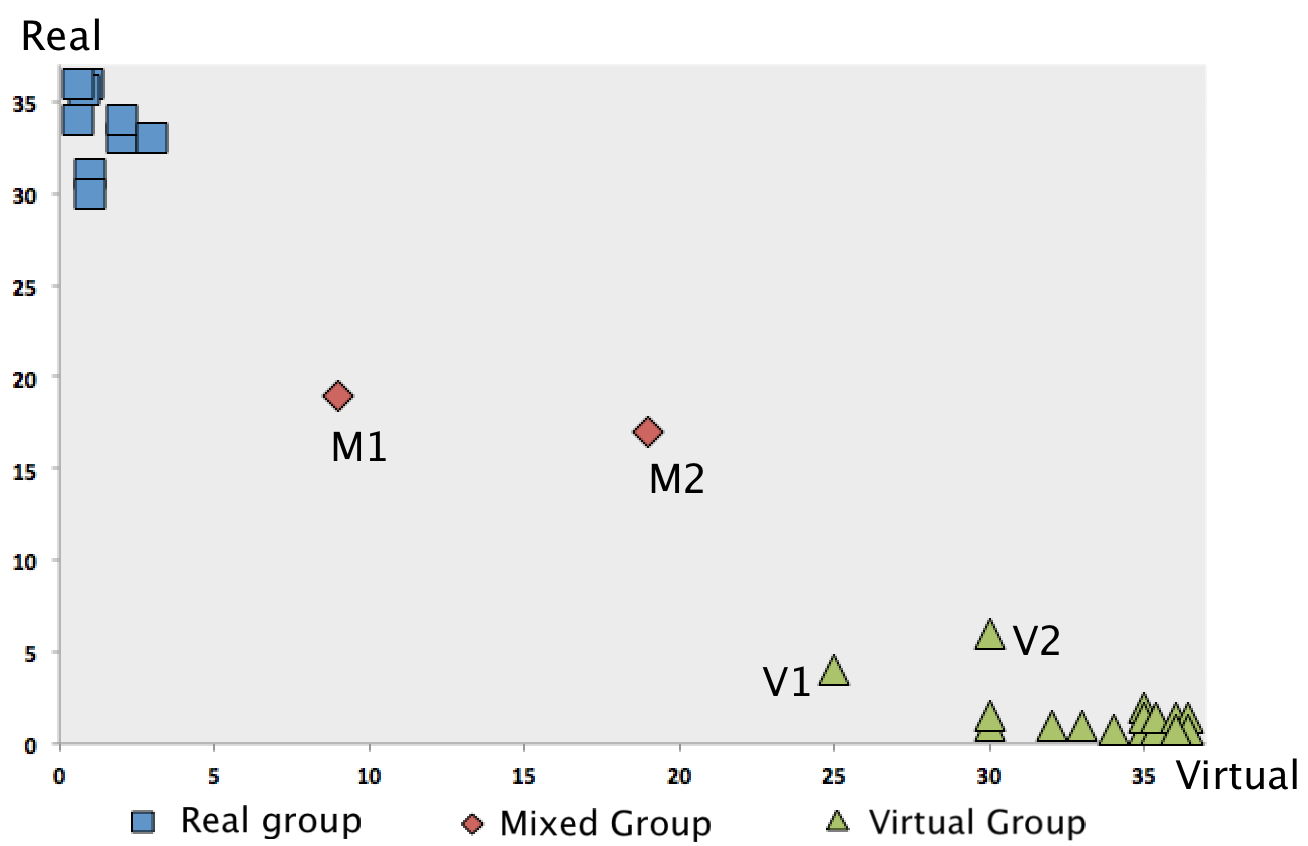
\includegraphics[width=\textwidth]{figures/2_clustering}
  \caption{\label{fig:2_clustering}The distribution of participants according to their number of choices on the virtual (avatar) and real (the experimenter) reference frames.}
\end{figure}

\begin{figure}[ht]
  \centering
  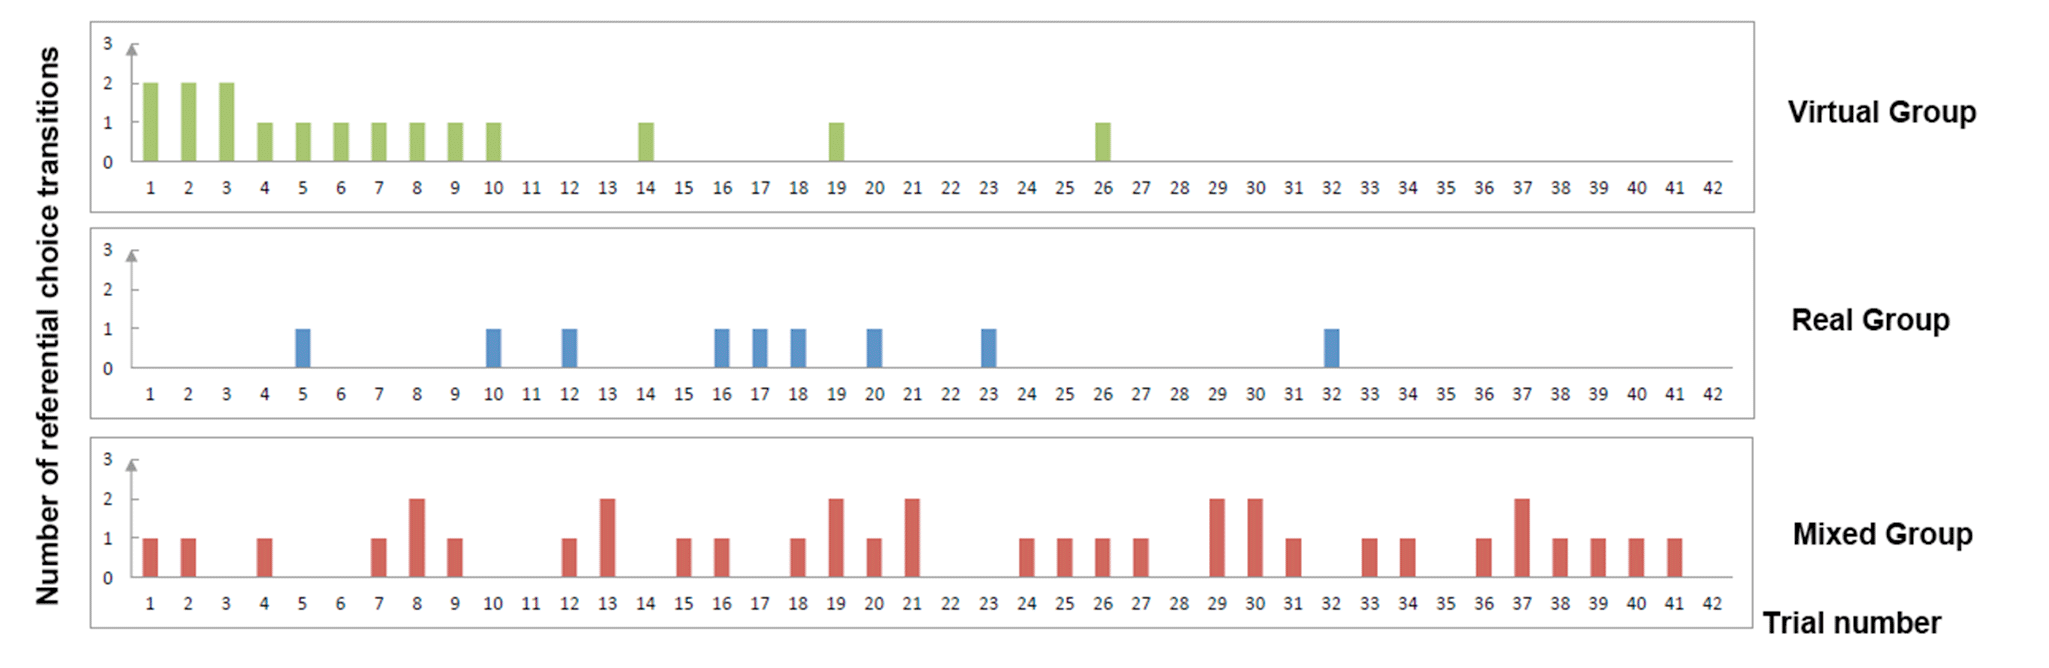
\includegraphics[width=\textwidth]{figures/2_transition}
  \caption{\label{fig:2_transition}Distribution of the number of collaborator choice transitions for each group.}
\end{figure}

From Figure~\ref{fig:2_transition}, we can get a global view of the difference between the three groups by counting the number of referential choice transitions in each trial. A referential choice transition occurs when a participant modifies his/her reference frame (Real to Virtual, or vice versa). For each trial, the number of transitions corresponds to the number of participants having such transition.

In the Virtual and Real groups, participants chose, from time to time, a reference frame which was not relevant for their group: the experimenter for the Virtual group, her avatar for the Real group. In these groups, the number of transitions was quite low if we compare it with the maximum value that it could reach (group size). For the Mixed group, we chose as baseline the virtual referential, so that what was shown in the graph was the number of participants who switched from the avatar toward the experimenter.

Anyway, since there were only two participants in the Mixed group, this group was not included for the comparison between groups in the following sections.

\subsubsection{Performance}
We applied the Kolmogorov-Smirnov test to verify if variables satisfy normality assumptions. All three behavioral variables failed the test: Reaction time (RT), K-S d = 0.21467, p \textless{} 0.01; Execution time (ET) K-S d = 0.17533, p \textless{} 0.01; Total time (TT) K-S d = 0.16585, p \textless{} 0.01. Therefore we used a non-parametric Kruskal–Wallis ANOVA test with delocalization angle and instruction type as inter-trial factors. For Post hoc analyses, we used multiple comparisons of mean ranks for all groups.

\paragraph{Global analyses}
Regarding task efficiency (RT – Reaction Time, ET - Execution Time, TT – Total Time), first we examined the influence of delocalization angle (Table~\ref{tab:angles}) and we found a main effect on the ET (H (6, N=1079) = 20.51355, p = 0.002) and TT (H (6, N=1079) = 18.68352, p = 0.004). Post hoc comparisons showed that participants spent more time to execute the task with angle 180$^{\circ}$ than with 0$^{\circ}$, 30$^{\circ}$ and 90$^{\circ}$. For TT, participants spent more time to complete the task with angle 180$^{\circ}$ than with angle 0$^{\circ}$ (Figure~\ref{fig:2_angles}).

\begin{table*}[!t]
\renewcommand{\arraystretch}{1.3}
\caption{Mean value and standard deviation of reaction time (RT), execution time (ET) and total time (TT) for each delocalization angle.}
\label{tab:angles}
\centering
\begin{tabular}{p{2.5cm} l l l l l l}
	\hline
     & \multicolumn{2}{p{3cm}}{Reaction Time} & \multicolumn{2}{p{3cm}}{Execution Time} & \multicolumn{2}{p{3cm}}{Total Time} \\
     Delocalization Angle & \multicolumn{2}{p{2.5cm}}{(millisecond)} & \multicolumn{2}{p{2.5cm}}{(millisecond)} & \multicolumn{2}{p{2.5cm}}{(millisecond)} \\
    (degree) & Mean & SD & Mean & SD & Mean & SD \\
    \hline
    0 & 1482 & 1062 & 1592 & 607 & 3074 & 1263 \\
   	30 & 1779 & 1543 & 1646 & 755 & 3425 & 1905 \\
	60 & 1570 & 966 & 1698 & 784 & 3268 & 1271 \\
	90 & 1633 & 1188 & 1599 & 629 & 3232 & 1520 \\
	120 & 1764 & 1746 & 1606 & 613 & 3370 & 1949 \\
	150 & 1946 & 1901 & 1852 & 1000 & 3798 & 2336 \\
	180 & 1770 & 1508 & 1891 & 972 & 3661 & 1754 \\ \hline
\end{tabular}
\end{table*}

Second we checked the relationship between task efficiency and instruction type, and we found a main effect on RT (H (2, N=1078) = 86.98551, p = 0.00001) and TT (H (2, N=1079) = 41.48673, p = 0.00001). Post hoc comparisons showed that gesture-only instructions required the most time and the results were intermediate with multimodal instructions (Figure~\ref{fig:2_instruction}).

\begin{figure}[ht]
  \centering
  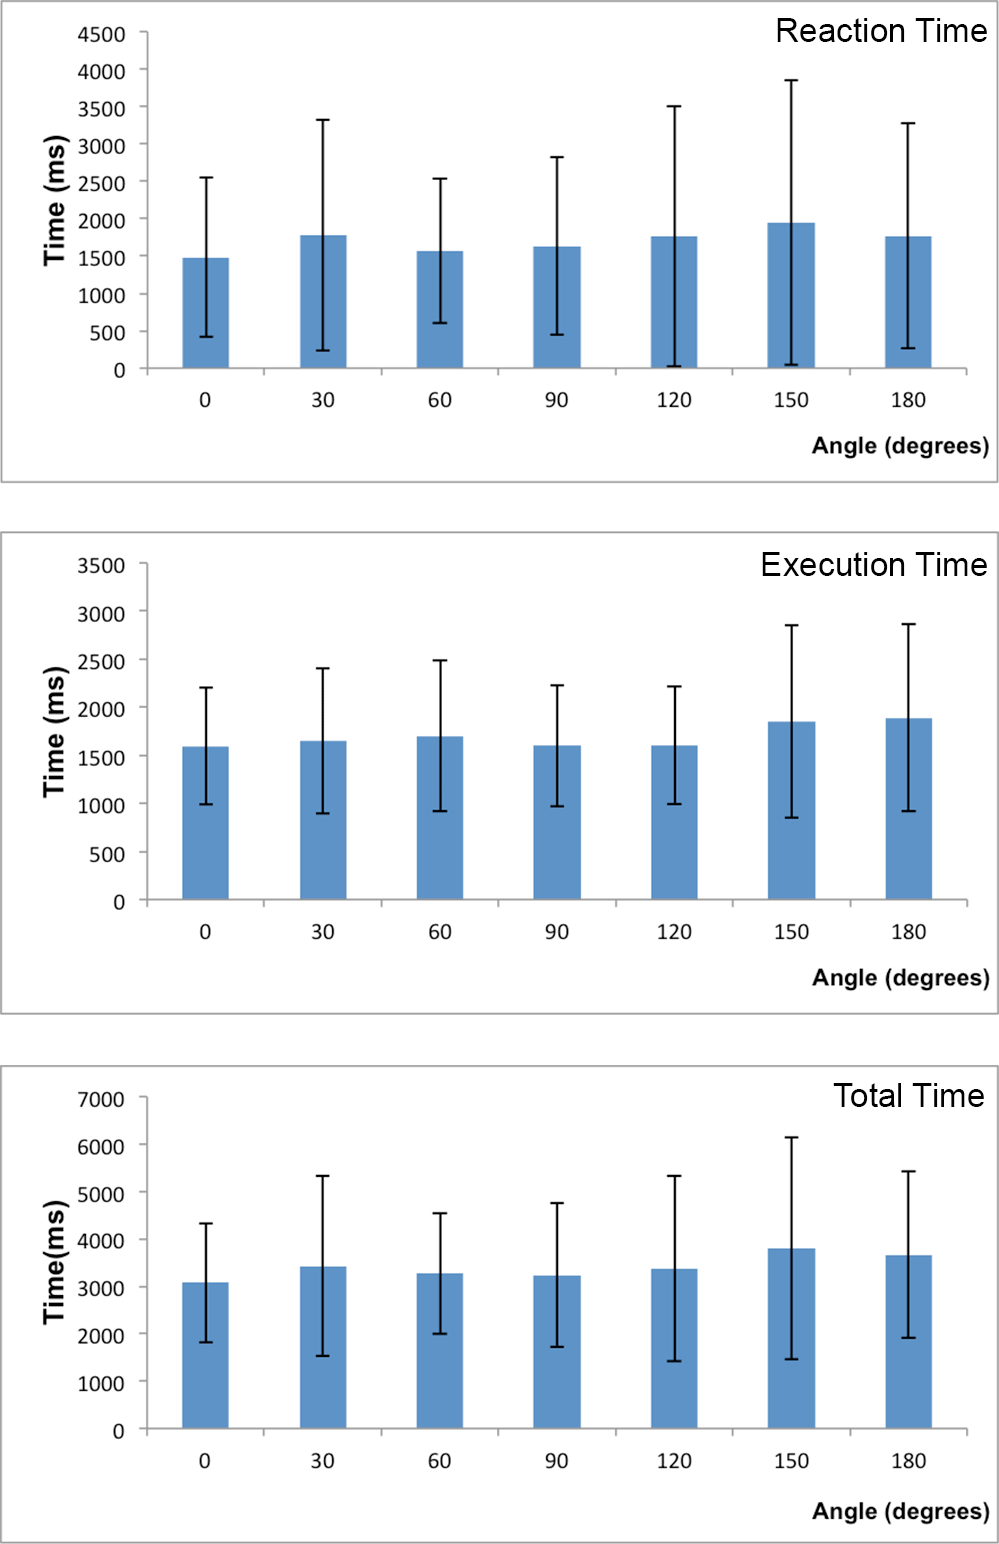
\includegraphics[width=\textwidth]{figures/2_angles}
  \caption{\label{fig:2_angles}Mean value and standard deviation of reaction time (RT), execution time (ET), and total time (TT) for each delocalization angle.}
\end{figure}

\begin{figure}[ht]
  \centering
  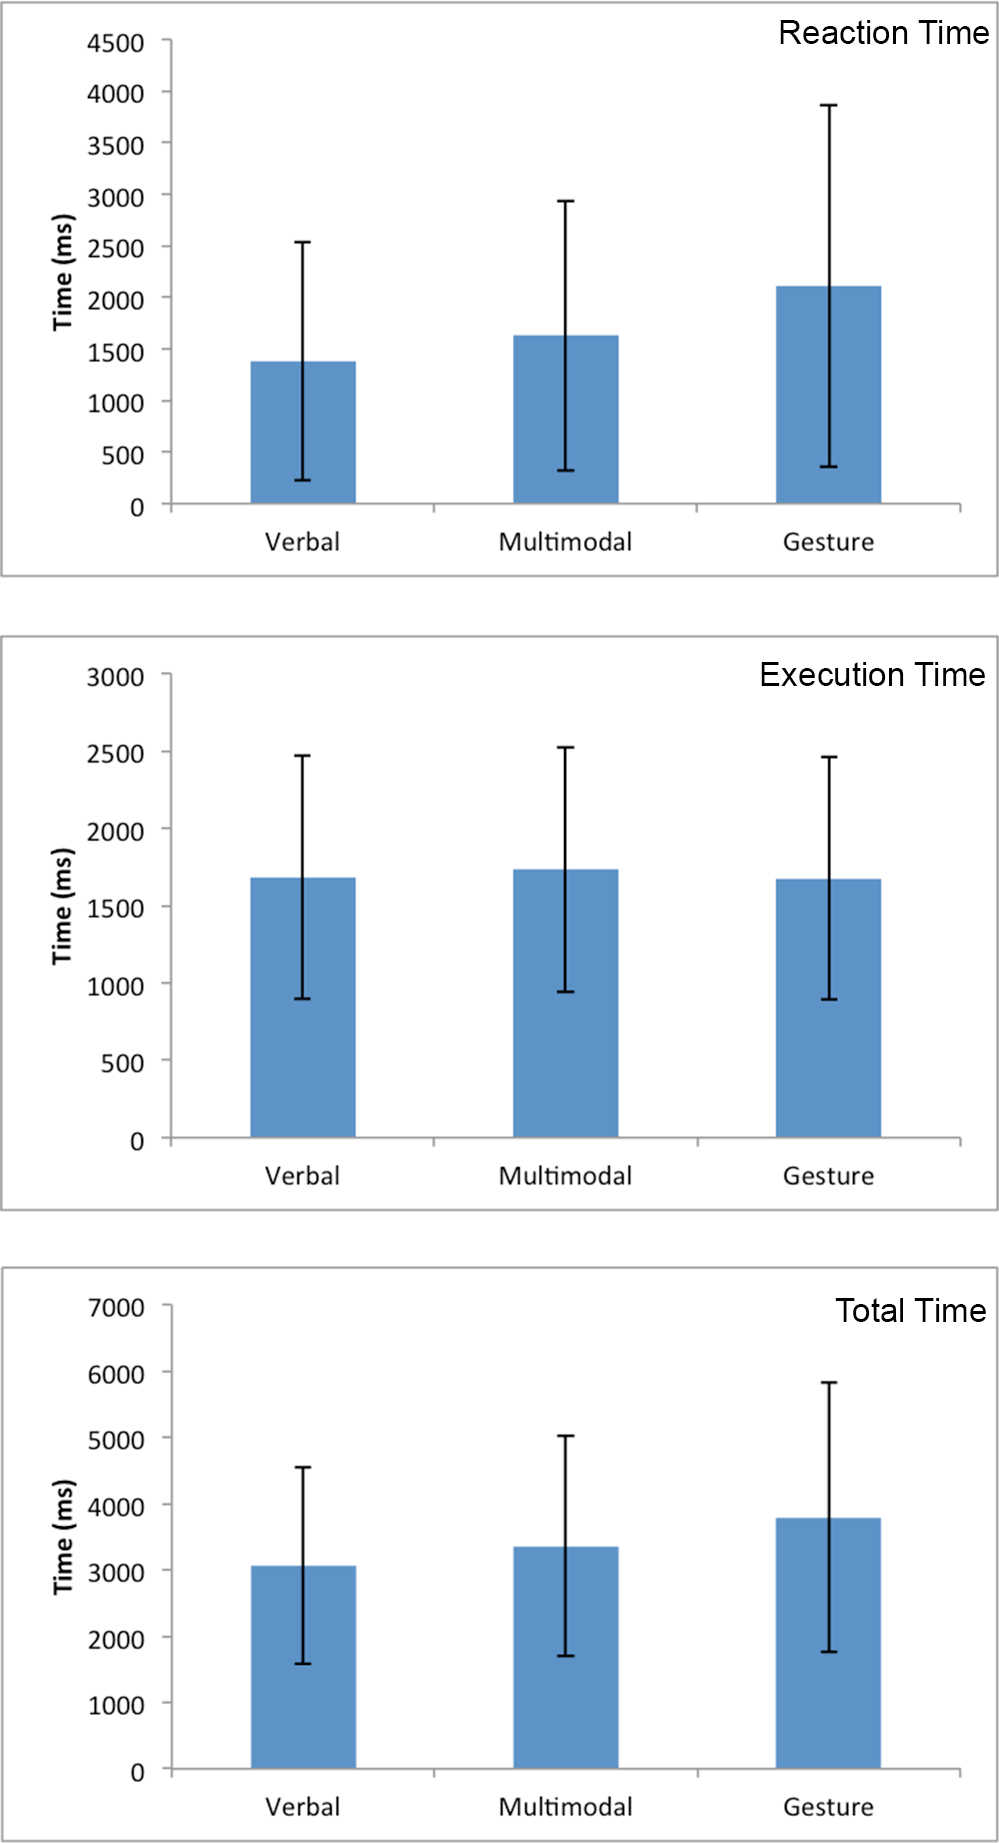
\includegraphics[width=\textwidth]{figures/2_instruction}
  \caption{\label{fig:2_instruction}Mean value and standard deviation of reaction time (RT), execution time (ET), and total time (TT) for each type of instruction.}
\end{figure}

\begin{table*}[!t]
\renewcommand{\arraystretch}{1.3}
\caption{Mean value and standard deviation of reaction time (RT), execution time (ET) and total time (TT) for each type of instruction.}
\label{tab:metrics}
\centering
\begin{tabular}{l l l l l l l}
	\hline
    & \multicolumn{2}{p{3cm}}{Reaction Time} & \multicolumn{2}{p{3cm}}{Execution Time} & \multicolumn{2}{p{3cm}}{Total Time} \\
    Instruction Type & \multicolumn{2}{p{3cm}}{(millisecond)} & \multicolumn{2}{p{3cm}}{(millisecond)} & \multicolumn{2}{p{3cm}}{(millisecond)} \\
    \hline
    & Mean & SD & Mean & SD & Mean & SD \\
    Verbal & 1384 & 1157 & 1682 & 785 & 3065 & 1481 \\
	Multimodal & 1627 & 1306 & 1731 & 789 & 3358 & 1658 \\
	Gesture & 2113 & 1755 & 1677 & 785 & 3790 & 2036 \\ \hline
\end{tabular}
\end{table*}

\paragraph{Inter-group analysis}
We measured the influence of delocalization angle and instruction type in each group separately to see if they had an effect on a certain population.

For the Real group, we got a main effect of instruction type on RT (H (2, N=364) = 27.10793, p \textless{} 0.000001) and TT (H (2, N=364) = 10.5341, p = 0.005). Post hoc comparisons showed that participants spent more time to react and to finish the task with gesture-only instructions than with the other two types of instruction while multimodal instructions were at a medium level.

For the Virtual group, a main effect of instruction type was also found on RT (H (2, N = 640) = 60.62227, p \textless{} 0.000001) and TT (H (2, N=641) = 32.36614, p \textless{} 0.000001). Post hoc comparisons showed the same result as for the Real group.

\subsubsection{Subjective data}
\paragraph{Global analyses}
We gathered participants' subjective feelings as a complement to performance measures. First we used the SSQ to see possible occurrence of cybersickness after the exposure to the experimental perceptual conflicts. Then we extracted some descriptive results (e.g., confidence feeling, etc) from the subjective questionnaire.

The simulator sickness was assessed before and after the experimental session using the SSQ. We found that the scores (by subtracting the pre-experimental measures to post-experimental measures) to the various sub-scales are relatively low. To study the impact of such immersive system (i.e., simulator effect), we applied the Kolmogorov-Smirnov test to verify that the variables failed to satisfy normality assumptions (Pre-score: K-S, d = 0.25607, p \textless{} 0.05; Post-score: K-S, d = 0.29235, p \textless{} 0.01). So we computed a Wilcoxon signed rank test on two paired samples on the pre (Mean = 164.21, SD = 221.34) and post (Mean = 155.02, SD = 212.07) scorings of SSQ. No effect of cybersickness was found after the experiment (N = 17, T = 68, Z = 0.402373908, p = 0.687409138).

From the subjective questionnaire, we found that the participants were moderately confident in their success of tasks and they felt only a little nervous about the dual-presence during the collaboration (Table~\ref{tab:sub_qn}).

\begin{table*}[!t]
\renewcommand{\arraystretch}{1.3}
\caption{Global result of the subjective questionnaire for all participants.}
\label{tab:sub_qn}
\centering
\begin{tabular}{l l l l}
	\hline
	Item & Mean & SD & Range \\ \hline
	Confidence of task success & 29.00 & 5.46 & [0, 40] \\
	Instruction understanding & 15.76 & 6.39 & [0, 28] \\
	Ease of dual-presence & 16.92 & 5.32 & [0, 36] \\
	Experience with virtual environment (VE) & 1.76 & 1.36 & [0, 4] \\
	Experience with Virtual Reality (VR) & 1.24 & 1.27 & [0, 4] \\
	Experience with video games & 2.08 & 1.00 & [0, 4] \\ \hline
\end{tabular}
\end{table*}


\paragraph{Inter-group analyses}
We conducted inter-group comparison to check the relationship between the participants' collaborator choice and their individual characteristics. Regarding the simulator sickness, with Wilcoxon signed rank test on two paired samples, no matter in which group, participants did not experience cybersickness (Virtual group: N = 16, T = 20.5, Z = 0.236939551, p = 0.812703838; Real group: N = 9, T = 11.5, Z = 0.422577127, p = 0.672604101).

We used the Student's t-test with subjective questionnaire responses as inter-subject variables to compare the Real and Virtual group. We found a main effect on instruction understanding between participants in the Virtual group and those in the Real group (Table~\ref{tab:inter_gp_sub_qn}). Participants in the Real group declared weaker instruction understanding than participants in the Virtual group (Figure~\ref{fig:2_subjective_qn}). We also found an effect on user's video game experience. Participants in the Virtual group played video games more often than those in the Real group (Table~\ref{tab:inter_gp_sub_qn}).

\begin{figure}[ht]
  \centering
  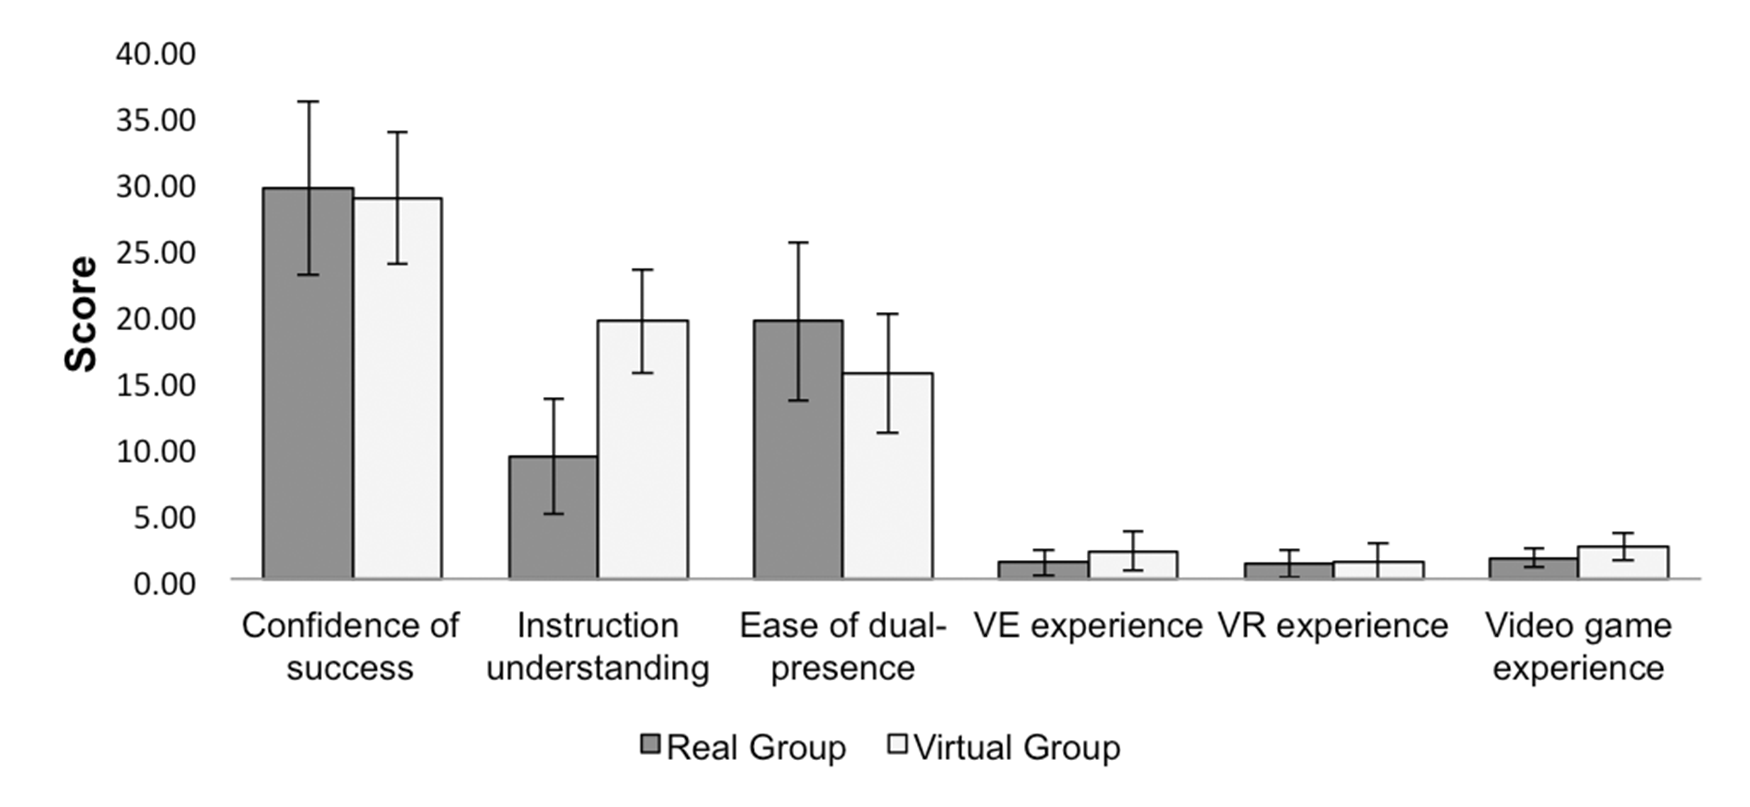
\includegraphics[width=\textwidth]{figures/2_subjective_qn}
  \caption{\label{fig:2_subjective_qn}Comparison of Real and Virtual groups according to the result of the subjective questionnaire.}
\end{figure}

\begin{table*}[!t]
\renewcommand{\arraystretch}{1.3}
\caption{Mean value and standard deviation of the result of subjective questionnaire and result of Student test between the Real group and Virtual group.}
\label{tab:inter_gp_sub_qn}
\centering
\begin{tabular}{l l l l l l l}
	\hline
    Item & \multicolumn{2}{p{2.8cm}}{Real group} & \multicolumn{2}{p{2.8cm}}{Virtual group} & \multicolumn{2}{p{3cm}}{Between groups} \\ \cline{6-7}
    & Mean & SD & Mean & SD & Student test & p-value \\ \hline
    Confidence of success & 29.44 & 6.54 & 28.75 & 4.97 & t(23) = -0.30 & 0.77 \\
	Instruction understanding & 9.22 & 4.32 & 19.44 & 3.90 & t(23) = 6.05 & \textbf{0.000004} \\
	Ease of dual-presence & 19.44 & 6.00 & 15.50 & 4.49 & t(23) = -1.87 & 0.07 \\
	VE experience & 1.22 & 0.97 & 2.06 & 1.48 & t(23) = 1.52 & 0.14 \\
	VR experience & 1.11 & 1.05 & 1.31 & 1.40 & t(23) = 0.37 & 0.71 \\
	Video game experience & 1.56 & 0.73 & 2.38 & 1.02 & t(23) = 2.11 & \textbf{0.046} \\ \hline
\end{tabular}
\end{table*}

\subsection{Discussion}
In the absence of instructions to impose the participants to collaborate with the avatar in our experiment, we left the participants to choose between the real or virtual collaborator. In the experimental scenario that we created, a virtual object was always present in the pointing direction of the real experimenter so the real pointing gesture became meaningful. According to the result, the physical presence of the experimenter both in the visual and audio modalities appeared to cause a significant proportion of participants to choose the real person instead of the avatar. In fact, 33\% of all participants chose to work with the real experimenter and ignored the animated avatar. Meanwhile the rest (59\%) interacted successfully with the avatar. So our hypothesis on participants' choice of collaborator (H1) was rejected. Three of those who finally chose the avatar have asked ``Whom should I work with?" and we told them ``Do as you like". However, none of the participants in the Real or Mixed group asked this question.

Moreover, almost all users made their choice in the early stage of the experiment, which either stayed stable during all trials or was gradually stabilized from trial to trial (especially participants V1 and V2 in Figure~\ref{fig:2_clustering}). Only the two users from the Mixed group (the participants M1 and M2 oscillated between the real experimenter and the avatar from the beginning to the end of the experiment (Figure~\ref{fig:2_transition}). This result was corroborated by the fact that the collaborator choice was not significantly impacted by delocalization angle or by the instruction type. However, inter-group comparisons showed that participants' familiarization with video games had a significant impact on their collaborator choice. Participants who chose the avatar were those who played more video games. The results of the subjective questionnaire also indicated that participants in the Real group had problems understanding the instructions compared to those in the Virtual group.

Regarding the impact of different experimental conditions on task performance, we first assumed that the spatial proximity of the collaborator and the avatar should provide stronger visual conflicts and thus would take the participants longer time to accomplish the task. Actually, this hypothesis (H2) was also rejected. There were no significant results confirming that small angle were more disturbing than larger ones. The distance between the real experimenter and her avatar did not seem to have an influence on participants' decision making. This may be the result of the co-effect of visual conflicts (Figure~\ref{fig:2_inconsistency}(a)) and audio-visual inconsistency (Figure~\ref{fig:2_inconsistency}(b)). Larger delocalization angle may cause weaker visual conflicts, but the audio-visual inconsistency will become stronger. Further studies are needed to separate these two factors (e.g., spatialized audio can be used to map the audio source to the avatar) and to investigate their individual influence on task performance.

Then for the comparison of different instruction types, overall participants had the best performance with verbal-only instruction (M = 1384, SD = 1157), and the weakest performance with gesture-only instruction (M = 2113, SD = 1755), while the multimodal instruction was medium (M = 1627, SD = 1306). This result confirmed our hypothesis on the influence of instruction modality on task performance (H3) that participants should be more efficient with verbal-only instructions than with instructions that involve gestural information when facing the dual-presence of the experimenter.

Unimodal commands like deictic gestures (pointing) or speech usually have an ambiguity problem \citep{Bangerter2004Using}. For example, pointing precision depends on the distance between hand and target, the density of objects in the pointing zone, etc. The efficiency of verbal command also varies according to the task and context. In our crown-picking task, these ambiguities were removed by asking participants to pick the nearest crown next to the experimenter, so the reaction time for different types of instructions depended on the time that the participants needed to receive and process the information. Studies on human reaction to visual-auditory stimuli have shown that humans have similar reaction time for auditory and visual stimuli (around 392 milliseconds) \citep{Suied2009Integration} or are slightly quicker with auditory (284 milliseconds) than visual (331 milliseconds) stimuli \citep{Shelton2010Comparison}. To process information conveyed in the instructions, relational expressions in verbal instructions like ``Go to the crown on my left" required the participants to rely on an allocentric reference frame with spatial updating abilities \citep{Riecke2007Spatial}, whereas pure pointing gestures can be handled within participants' egocentric reference frame. So normally participants should be quicker with gestural instructions than with verbal instructions because the former did not require participants to do mental rotations which may take several seconds depending on the rotation angle \citep{Shepard1971Mental}. Additionally, multimodal systems usually provide better task efficiency compared to unimodal systems in spatial domains \citep{Oviatt1999Ten}. The opposite result (i.e., the user spent less time with verbal instructions than with multimodal and gestural ones) that we observed in our experiment can be explained by the fact that participants were disturbed by the visual conflict induced by the dual-presence of the experimenter and this visual conflict was enhanced by the pointing gesture.

\subsection{Summary}
As the results showed, first users had an a priori choice of collaborator (avatar or real person) and this choice did not change under different experimental conditions. Second, perceptual conflicts had an impact on users' performance in term of task completion time. We discuss the implications of these results for designing a better immersive system for co-located collaboration between multiple users.

The goal of this paper was to study user behavior and performance influenced by simultaneous real and virtual stimuli coming from an experimenter and her avatar (dual-presence) in a collaborative virtual context offered by multi-stereoscopic projection-based immersive device. In a two-user scenario, participants performed an object-picking task according to three types of instructions (verbal-only, gesture-only or multimodal instructions) given by an experimenter and her avatar which was delocalized from the real person according to a regular distribution of rotation angles (greater the angle, farther the experimenter and her avatar).

We found that most users had an a priori choice of collaborator, which stayed stable through all trials (neither the delocalization angle nor the instruction type had an influence on this choice). 33\% of participants chose to interact with the real experimenter, 59\% of participants worked with the avatar, while the rest remained undecided. This choice may be the result of combined effects of many factors, for example, user's experience with video games, the quality of the visual display, the reactiveness of the motion tracking system, etc.

When a user faced the dual-presence of another co-located user, it seemed that the cognitive process helped him/her to solve the perceptual conflicts and allowed him/her to follow a coherent strategy. However, it was at a cost of task performance for instructions that involved gesture information.

\section{Conclusion}

All these results provided us three possible research axes to design effective solutions to manage co-located collaboration in multi-stereoscopic immersive systems. First, in future experiments or applications we can explicitly ask users to follow the virtual representation (the avatar) of the experimenter despite their perception of the dual-presence. It would be interesting to observe the reaction of users and to compare their performance with the results of the experiment presented in this paper, especially for users who were in the Real and Mixed group. Second, tasks that require more complicated interactions and have longer duration between collaborators could be tested (with pairs of experimenter and participant, or pairs of participants) to further investigate the impact of certain factors (e.g., delocalization angle) on task performance. At last, as we observed that the dual-presence brought conflicting information in the visual channel and thus reduced user performance for instructions including gestural interactions, an important issue could be to propose scene management approaches to limit the visual duality (i.e., visual perception of real user and his/her avatar). We could also add some automatic control (e.g., redirections) to the avatar-based approach to prevent co-located users from seeing each other's real body when navigating in the virtual world so as to avoid the perception of dual-presence.
